\documentclass[12pt, a4paper]{article}
\usepackage[utf8]{inputenc}
\usepackage[brazilian]{babel}
\usepackage[T1]{fontenc}
\usepackage{graphicx}
\usepackage{geometry}
\usepackage{color,soul}
\usepackage[document]{ragged2e}
\usepackage{float}
\usepackage{setspace}
\usepackage{indentfirst}
\usepackage[normalem]{ulem}


% ---
% Informações que podem ser configuradas (MACROS)
% ---
\newcommand{\class}{Universidade de Brasilia, Faculdade do Gama} % Nome da disciplina
\newcommand{\term}{2019.1}                                       % Perído Letivo
\newcommand{\examnum}{Sistema de Bancos de Dados 1}              % Número/Nome do exercício.
\newcommand{\estudant}{Welison Lucas A. Regis}
\newcommand{\register}{17/0024121}
% \newcommand{\examdate}{19/03/2019}                               % insere a data no documento
% \newcommand{\tf}[1][{}]{                                         % Para questões de verdadeiro ou falso
%     \fillin[#1][0.25in]
% }

% ---
% Diagramação
% ---
\geometry{top=2.5cm, bottom=2.0cm, right=2.0cm, left=2.5cm}
\onehalfspacing

% ---
% COMEÇO DO DOCUMENTO
% ---
\begin{document}



% \thispagestyle{empty} % deixa de enumerar a página

% ---
% LOGO UNB
% ---
\begin{figure}
    \centering
    
\includegraphics[width=1.0\linewidth, height=1.2cm]{images/as_comp_PB.jpg}
    \vspace{-1.5em}    
    \label{unb:unb_logo}
\end{figure}

% ---
% CABEÇALHO
% ---
\noindent
\begin{tabular*}{\textwidth}{l @{\extracolsep{\fill}} r @{\extracolsep{6pt}} l}
\textbf{\class} & \textbf{Nome:} & \textit{\estudant}\\
\textbf{\term} & \textbf{Matricula:} & \textit{\register}\\
\textbf{\examnum} &&\\
\end{tabular*}\\
\rule[2ex]{\textwidth}{2pt}


% ---
% TÍTULO
% ---
\begin{center}
    \vspace{-1.5em}
    \textbf{\Large{Exercício - Instituição Financeira}}
\end{center}
\rule[2ex]{\textwidth}{2pt}
\vspace{-3em}

% ---
% CONTEÚDO
% ---

% Texto justificado e com identação de 1,5cm
\justify
\setlength{\parindent}{1.5cm}

% ---
% MER
% ---
\section{MODELO ENTIDADE RELACIONAMENTO}

\subsection{Entidades}

\par CLIENTE
\par ENDERECO
\par AGENCIA
\par CONTA
\par \hspace{1.5cm} CONTA\_CORRENTE
\par \hspace{1.5cm} CONTA\_POUPANCA
\par \hspace{1.5cm} CONTA\_INVESTIMENTO
\subsection{Atributos}

\par CLIENTE(\underline{cpf}, nome, idEndereco, email, \{telefone\})
\par ENDERECO(\underline{idEndereco}, numero, logradouro, bairro, cidade, uf, cep, complemento)
\par AGENCIA(\underline{numeroAgencia}, idEndereco, telefone, email)
\par CONTA(\underline{numeroConta}, \underline{numeroAgencia}, saldo, cpf)

\par \hspace{1.5cm} CONTA\_CORRENTE(limiteChequeEspecial)
\par \hspace{1.5cm} CONTA\_POUPANCA(dtAniversario, juroMensal)
\par \hspace{1.5cm} CONTA\_INVESTIMENTO(rendimentoDiario)

\subsection{Relacionamentos}

CLIENTE - \textbf{possui} - ENDERECO: um CLIENTE possui um endereço, assim como um ENDERECO pode pertencer a um ou mais cliente(s). Cardinalidade: \textbf{1 : n}.

CLIENTE - \textbf{possui} - CONTA: um CLIENTE possui uma ou várias conta(s), porém, uma CONTA pertence a apenas um cliente. Cardinalidade: \textbf{1 : n}.

AGENCIA - \textbf{tem} - CONTA: uma AGENCIA tem uma ou muitas conta(s), já uma CONTA pertence a apenas uma agência. Cardinalidade: \textbf{1 : n}.

AGENCIA - \textbf{tem} - ENDERECO: uma AGENCIA tem apenas um endereço, assim como um ENDERECO pertence a apenas uma agência. Cardinalidade: \textbf{1 : 1}.




% ---
% DER
% ---
\section{DIAGRAMA ENTIDADE RELACIONAMENTO}

\begin{figure}[H]
    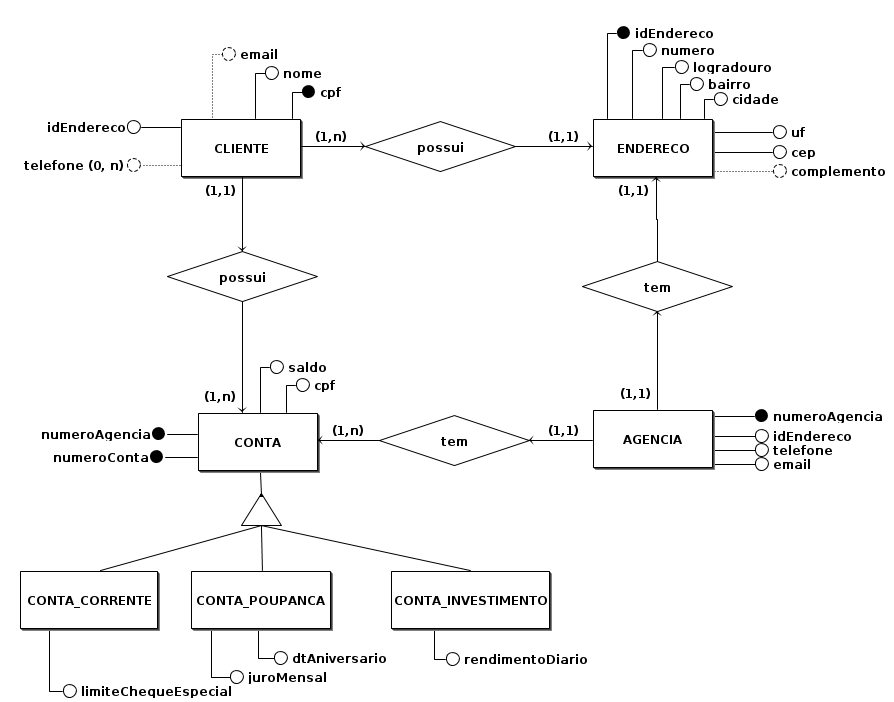
\includegraphics[width=\linewidth]{images/DER.png}
    \caption{DER — representação das entidades, atributos e relacionamentos}
    \label{fig:diagrama}
\end{figure}

\newpage



% ---
% DE
% ---
\section{DIAGRAMA DE ESQUEMA}

\begin{figure}[H]
    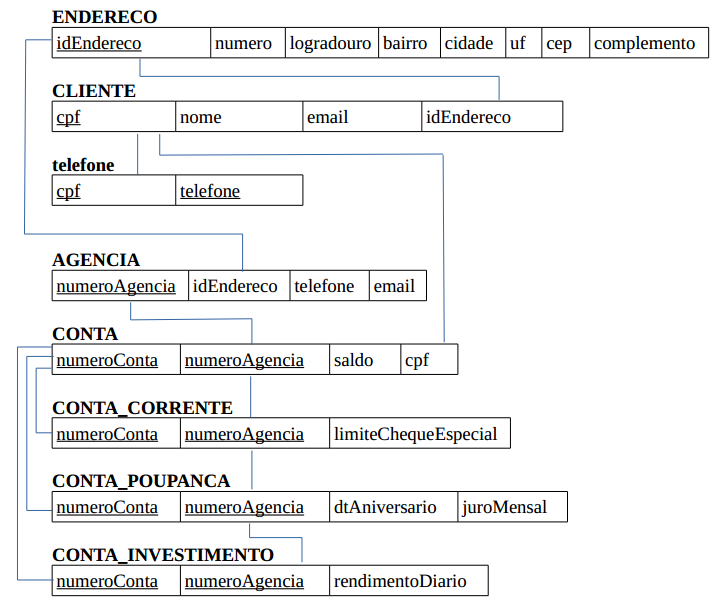
\includegraphics[width=\linewidth]{images/DE.png}
    \caption{Diagrama de Esquema}
    \label{fig:diagrama2}
\end{figure}

\newpage



\end{document}
